\documentclass[french]{article}
\usepackage[T1]{fontenc}
\usepackage[utf8]{inputenc}
\usepackage[french]{babel}
\usepackage{amsmath}
\usepackage{mathtools}
\usepackage{color}
\usepackage[svgnames,dvipsnames]{xcolor} 
\usepackage{soul}
\usepackage{amssymb}
\usepackage{enumitem}
\usepackage{multicol}
\usepackage[left=2cm,right=2cm,top=2cm,bottom=2cm]{geometry}
\newcommand{\mathcolorbox}[2]{\colorbox{#1}{$\displaystyle #2$}}
\usepackage{pifont}
\usepackage{pst-all}
\usepackage{pstricks}
\usepackage{delarray}
\usepackage{setspace}
\usepackage{graphicx}
\usepackage{hyperref}
\usepackage{nicematrix}
\usepackage{listings}
\usepackage{float}

\hypersetup{
	colorlinks=true,
	linkcolor=blue,
	filecolor=magenta,      
	urlcolor=cyan,
	pdfpagemode=FullScreen,
}

\usepackage{amsthm}
\newtheorem*{Rem}{Remarque}

\newenvironment{conclusion}[1]{%
	\begin{center}\normalfont\textbf{Conclusion}\end{center}
	\begin{quotation} #1 \end{quotation}
}{%
	\vspace{1cm}
}

\lstset{language=C++,
	basicstyle=\ttfamily,
	keywordstyle=\color{blue}\ttfamily,
	stringstyle=\color{red}\ttfamily,
	commentstyle=\color{green}\ttfamily,
	morecomment=[l][\color{magenta}]{\#}
}

\setlength\parindent{0pt}
\allowdisplaybreaks
\newcommand\numberthis{\addtocounter{equation}{1}\tag{\theequation}}

\begin{document}
	LECOURTIER Frédérique \hfill \today
	\begin{center}
		\Large\textbf{{Explication - Résultats similaires avec les 2 méthodes de correction.}}\\
	\end{center}
	\graphicspath{{images/}}
	
	On considère le problème de Poisson avec condition de Dirichlet homogène ou non homogène :
	\begin{equation}
		\label{pb1}
		\left\{\begin{aligned}
			&-\Delta u=f \quad &&\Omega \\
			&u=g \quad &&\Gamma
		\end{aligned}\right. \tag{$\mathcal{E}_1$}
	\end{equation}
	
	On a ainsi une EDP que l'on souhaite résoudre sur un domaine $\Omega$. On note $\Gamma$ le bord de $\Omega$, c'est-à-dire $\Gamma=\partial\Omega$. 
	
	Dans notre cas, on souhaite appliquer une correction à la sortie d'un FNO.
	On considère ici que l'on possède une solution analytique $u$ et qu'après une utilisation du FNO, on obtient une solution du type
	\begin{equation*}
		\label{phi_tild}
		\tilde{\phi}(x,y)=u_p(x,y) = u(x,y)-\epsilon P(x,y)
	\end{equation*}
	avec $P$ la perturbation (tel que $P=0$ sur $\Gamma$) et $\epsilon$ petit.
	
	Ce document a pour but de comparer deux méthodes de correction de ce problème :
	\begin{enumerate}[label=\textbullet]
		\item \textbf{Méthode 1 : }
		On souhaite résoudre le problème suivant
		\begin{equation}
			\label{pbc1}
			\left\{\begin{aligned}
				&-\Delta (\tilde{\phi}C)=f \quad &&\Omega \\
				&C=1 \quad &&\Gamma
			\end{aligned}\right. \tag{$\mathcal{C}_1$}
		\end{equation}
		
		avec $\tilde{u}=\tilde{\phi}C$.
		
		Dans un autre document, on a présenté l'intérêt de rehausser le problème et de se ramener au problème suivant
		
		\begin{equation}
			\left\{\begin{aligned}
				&-\Delta (\hat{\phi}C)=f \quad &&\Omega \\
				&\hat{u}=g+m \quad &&\Gamma
			\end{aligned}\right. \label{pbc1r} \tag{$\mathcal{C}_1^\mathcal{R}$}
		\end{equation}
		avec $\hat{u}=\hat{\phi}C+m$ où $\hat{\phi}=\tilde{\phi}+m$ ($m$ une constante).
		
		
		\item \textbf{Méthode 2 : } On souhaite résoudre le problème suivant
		\begin{equation}
			\label{pbc2}
			\left\{\begin{aligned}
				&-\Delta C=\tilde{f} \quad &&\Omega \\
				&C=0 \quad &&\Gamma
			\end{aligned}\right. \tag{$\mathcal{C}_2$}
		\end{equation}
		
		avec $\tilde{u}=\tilde{\phi}+C$ et $\tilde{f}=f+\Delta\tilde{\phi}$.
		
		\begin{Rem}
			On notera que dans ce cas rehausser le problème n'a aucun intérêt. \\
			En effet, la décomposition de $C_h$ sur la base $(\varphi_1,\dots,\varphi_{N_h})$ de $V_h$ s'écrit pour ce problème			
			$$C_h=\sum_{i=1}^{N_h}C_i\varphi_i$$
			avec $C_i=u(x_i)-\tilde{\phi}(x_i)$.
			Et donc, on a l'inégalité suivante
			$$||(u-\tilde{\phi})-C_h||_{L^2(\Omega)}\le ch^{k+1}|u-\tilde{\phi}|_{H^{k+1}(\Omega)}$$
			Alors
			$$|u-\tilde{\phi}|_{H^{k+1}(\Omega)}=||(u-\tilde{\phi})''||_{L^2(\Omega)}=||(\tilde{\phi}+\epsilon P-\tilde{\phi})''||_{L^2(\Omega)}=||P''||_{L^2(\Omega)}$$
			Et ainsi, en prenant $\hat{\phi}=\tilde{\phi}+m$ on obtient le même résultat.
		\end{Rem}
	\end{enumerate}

	\section*{Résultats numériques}
	
	On prend ici la solution analytique suivante
	$$u_{ex}(x,y) = S\times\sin(2\pi fx + p)\times\sin(2\pi fy + p)$$ 
	
	et $P$ la perturbation définie par
	$$P(x,y)=S\times\sin(2\pi f_px + p_p)\times\sin(2\pi f_py + p_p)$$
	
	avec $p_p=0$ pour que $P=0$ sur $\Gamma$ (et donc $u_p=u_{ex}$ sur $\Gamma$). 
	
	On cherche alors principalement à comparer les erreurs en norme $L^2$ obtenus avec les problèmes \ref{pbc1r} et \ref{pbc2}.
	
	On prendra $S=0.5$ et $p=0$ (c'est-à-dire $g=0$). On fera varier $\epsilon$, $f$ et $f_p$. 
	
	\newpage
	
	Voici les résultats obtenus :
	
	\begin{minipage}{\linewidth}
		\centering
		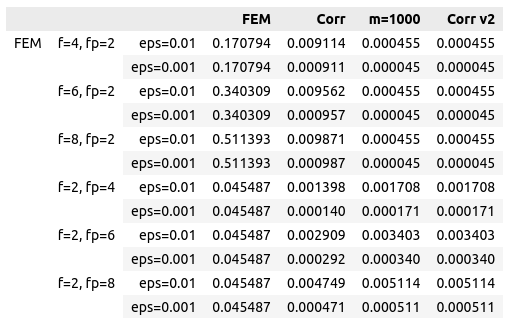
\includegraphics[width=0.55\linewidth]{resultats.png}
	\end{minipage}

	Il semblerait ici que les résultats obtenus pour les problèmes \ref{pbc1r} avec $m=1000$ (avant-dernière colonne) et \ref{pbc2} (dernière colonne) soient très proches.

	\section*{Explication}
	
	On cherche ici à comprendre pourquoi on obtient des résultats aussi proches avec les 2 méthodes.
	
	\subsection*{Méthode 1}
	
	On cherche à résoudre le problème
	\begin{equation}
		\left\{\begin{aligned}
			&-\Delta (\hat{\phi}C)=f \quad &&\Omega \\
			&\hat{u}=g+m \quad &&\Gamma
		\end{aligned}\right. \tag{$\mathcal{C}_1^\mathcal{R}$}
	\end{equation}
	avec $\hat{u}=\hat{\phi}C+m$ où $\hat{\phi}=\tilde{\phi}+m$ ($m$ une constante).
	
	La décomposition de $\hat{u_h}$ sur la base $(\varphi_1,\dots,\varphi_{N_h})$ de $V_h$ s'écrit pour ce problème
	
	\begin{equation}
		\hat{u_h}=C_h\hat{\phi}=\left(\sum_{i=1}^{N_h}C_i\varphi_i\right)\hat{\phi}(x) \label{decomp_pbc1}
	\end{equation}

	Or 
	\begin{equation}
		C_i=\frac{u(x_i)+m}{\hat{\phi}(x_i)}=\frac{u(x_i)+m}{\tilde{\phi}(x_i)+m} \label{C_i}
	\end{equation}
	avec
	\begin{equation}
		u(x_i)=\tilde{\phi}(x_i)+\epsilon P(x_i) \label{u_x_i}
	\end{equation}
	et
	\begin{equation}
		\tilde{\phi}(x)=\tilde{\phi}(x_i)+(x-x_i)\tilde{\phi}'(x_i) \label{phi_tilde_x}
	\end{equation}
	De plus
	\begin{equation}
		\sum_{i=1}^{N_h}\varphi_i=1 \label{sum_base}
	\end{equation}
	Avec les 4 relations précédentes, on peut développer \ref{decomp_pbc1} :
	\begin{align*}
		\hat{u_h}&=\left(\sum_{i=1}^{N_h}C_i\varphi_i\right)\hat{\phi}(x) \\
		&=\left(\sum_{i=1}^{N_h}\frac{u(x_i)+m}{\tilde{\phi}(x_i)+m}\varphi_i\right)\hat{\phi}(x) \quad \text{par \ref{C_i}} \\
		&=\left(\sum_{i=1}^{N_h}\frac{\tilde{\phi}(x_i)+m+\epsilon P(x_i)}{\tilde{\phi}(x_i)+m}\varphi_i\right)\hat{\phi}(x) \quad \text{par \ref{u_x_i}} \\
		&=\sum_{i=1}^{N_h}\left(1+\epsilon\frac{ P(x_i)}{\tilde{\phi}(x_i)+m}\right)\varphi_i\hat{\phi}(x) \\
		&=\left(\sum_{i=1}^{N_h}\varphi_i\right)\hat{\phi}(x)+\epsilon\sum_{i=1}^{N_h}P(x_i)\frac{\hat{\phi}(x)}{\tilde{\phi}(x_i)+m}\varphi_i \\
		&=\hat{\phi}(x)+\epsilon\sum_{i=1}^{N_h}P(x_i)\frac{\tilde{\phi}(x_i)+m+(x-x_i)\tilde{\phi}'(x_i)}{\tilde{\phi}(x_i)+m}\varphi_i \quad \text{par \ref{phi_tilde_x} et \ref{sum_base}} \\
		&=\hat{\phi}(x)+\epsilon\sum_{i=1}^{N_h}P(x_i)\left(1+\frac{(x-x_i)\tilde{\phi}'(x_i)}{\tilde{\phi}(x_i)+m}\right)\varphi_i \\
		&=\tilde{\phi}(x)+m+\epsilon\sum_{i=1}^{N_h}P(x_i)\left(1+\frac{(x-x_i)\tilde{\phi}'(x_i)}{\tilde{\phi}(x_i)+m}\right)\varphi_i \\
	\end{align*}

	Ainsi
	$$u_h=\hat{u_h}-m=\tilde{\phi}(x)+\epsilon\sum_{i=1}^{N_h}P(x_i)\left(1+\frac{(x-x_i)\tilde{\phi}'(x_i)}{\tilde{\phi}(x_i)+m}\right)\varphi_i$$
	et finalement
	\begin{equation}
		u_h\xrightarrow[m\to\infty]{} \tilde{\phi}(x)+\epsilon\sum_{i=1}^{N_h}P(x_i)\varphi_i \label{result1}
	\end{equation}
	
	
	\subsection*{Méthode 2}
	
	On cherche à résoudre le problème
	\begin{equation}
		\left\{\begin{aligned}
			&-\Delta C=\tilde{f} \quad &&\Omega \\
			&C=0 \quad &&\Gamma
		\end{aligned}\right. \tag{$\mathcal{C}_2$}
	\end{equation}
	avec $\tilde{u}=\tilde{\phi}+C$ et $\tilde{f}=f+\Delta\tilde{\phi}$.
	
	La décomposition de $u_h$ sur la base $(\varphi_1,\dots,\varphi_{N_h})$ de $V_h$ s'écrit pour ce problème
	
	\begin{equation}
		u_h=C_h+\tilde{\phi}=\left(\sum_{i=1}^{N_h}C_i\varphi_i\right)+\tilde{\phi}(x) \label{decomp_pbc2}
	\end{equation}
	
	Or 
	\begin{equation}
		C_i=u(x_i)-\tilde{\phi}(x_i) \label{C_i_2}
	\end{equation}
	avec
	\begin{equation}
		u(x_i)=\tilde{\phi}(x_i)+\epsilon P(x_i) \label{u_x_i_2}
	\end{equation}
	Avec les 2 relations précédentes, on peut développer \ref{decomp_pbc2} :
	\begin{align*}
		u_h&=\tilde{\phi}(x)+\sum_{i=1}^{N_h}C_i\varphi_i \\
		&=\tilde{\phi}(x)+\sum_{i=1}^{N_h}(u(x_i)-\tilde{\phi}(x_i))\varphi_i \quad \text{par \ref{C_i_2}} \\
		&=\tilde{\phi}(x)+\sum_{i=1}^{N_h}(\tilde{\phi}(x_i)+\epsilon P(x_i)-\tilde{\phi}(x_i))\varphi_i \quad \text{par \ref{u_x_i_2}} \\
		u_h&=\tilde{\phi}(x)+\epsilon\sum_{i=1}^{N_h} P(x_i)\varphi_i \numberthis \label{result2}
	\end{align*}
	
	Ainsi par \ref{result1} et \ref{result2}, il semblerait que pour le problème \ref{pb1}, les 2 méthodes proposées soit équivalentes (en prenant $m$ grand).

\end{document}